\pdfminorversion=5
\PassOptionsToPackage{colorlinks=true,allcolors=blue}{hyperref}
\documentclass[webpdf,contemporary,large]{oup-authoring-template}

\graphicspath{{figures/}}

% ---------------------------------------------------------------------------
% PRODUCTION CHECKLIST -- every item must be resolved before submission.
%   TODO-1  Author names, order, affiliations, ORCIDs, corresponding author.
%   TODO-2  Received / revised / accepted dates and DOI (publisher-supplied).
%   TODO-3  Funding statement and grant numbers.
%   TODO-4  Data availability: repository name, URL, accession numbers.
%   TODO-5  Code availability: GitHub tag/commit and Code Ocean capsule DOI.
%   TODO-6  Confirm public access and immutable versions of staged MIT code and weights.
% ---------------------------------------------------------------------------

\AtBeginDocument{%
  \hypersetup{%
    allcolors=blue
  }%
}

\newcommand{\figrefwhole}[1]{\hyperref[#1]{Figure~\ref*{#1}}}
\newcommand{\figpanelref}[2]{\hyperref[#1]{Figure~\ref*{#1}#2}}

\newcommand{\citewhole}[1]{%
  \hyperlink{cite.#1}{\NoHyper\citeauthor{#1}\endNoHyper, \NoHyper\citeyear{#1}\endNoHyper}%
}
\newcommand{\citewholep}[1]{%
  (\citewhole{#1})%
}

% Forward references into the companion Supplementary Material document.
\newcommand{\supfig}[1]{Supplementary Fig.~#1}
\newcommand{\suptab}[1]{Supplementary Table~#1}
\newcommand{\supsect}[1]{Supplementary Section~#1}

\usepackage{flafter,etoolbox}
% The original opening header adds a 4 mm bar/gap before a full-width inner box.
% Fit that inner box inside the existing text width; retain the original class file.
\makeatletter
\patchcmd{\ps@opening}{\vskip2.5pt\hbox to \textwidth}{\vskip2.5pt\hbox to \dimexpr\textwidth-4mm\relax}{}{\PackageError{CARBON}{Opening-header patch failed}{}}
\patchcmd{\ps@opening}{\vskip2.5pt\hbox to \textwidth}{\vskip2.5pt\hbox to \dimexpr\textwidth-4mm\relax}{}{\PackageError{CARBON}{Opening-header patch failed}{}}
\makeatother
\setlength{\emergencystretch}{1em}
\def\bibfont{\fontsize{7bp}{8.1bp}\selectfont}
\setlength{\textfloatsep}{8pt plus 2pt minus 2pt}
\setlength{\floatsep}{6pt plus 2pt minus 2pt}
\setlength{\intextsep}{6pt plus 2pt minus 2pt}
\setlength{\abovecaptionskip}{4pt plus 1pt minus 1pt}
\setlength{\belowcaptionskip}{0pt}
\renewcommand{\dblfloatpagefraction}{0.75}
\AtBeginDocument{\typeout{CARBON-LAYOUT: textwidth=\the\textwidth; columnwidth=\the\columnwidth; columnsep=\the\columnsep}}
\begin{document}
\linespread{0.96}\selectfont\raggedbottom

\journaltitle{Bioinformatics}
\DOI{DOI added during production}
\copyrightyear{YEAR}
\pubyear{YEAR}
\vol{XX}
\issue{x}
\access{Published: Date added during production}
\appnotes{Original Paper}

\firstpage{1}

\title[CARBON]{CARBON: a conservation-aware framework for base-resolution RBP binding profile prediction}

% TODO-1: replace the placeholder author block and affiliations.
% TODO-1: co-authors and the corresponding author are not yet decided.
% Author 1 (confirmed): Bin Wu, ORCID 0009-0002-6711-7230, College of Artificial
% Intelligence, Jilin University.  Replace the bracketed placeholders below
% before submission; the corresponding author e-mail must be supplied then.
\author[1]{Bin Wu\ORCID{0009-0002-6711-7230}}

\address[1]{\orgdiv{College of Artificial Intelligence}, \orgname{Jilin University}, \orgaddress{\street{2699 Qianjin Street}, \postcode{130012}, \state{Changchun}, \country{China}}}

\corresp[]{Corresponding author and e-mail to be confirmed.}

\received{Date}{0}{Year}
\revised{Date}{0}{Year}
\accepted{Date}{0}{Year}


\abstract{%
\textbf{Motivation:} Base-resolution RBP binding prediction requires both recognition of sequence preferences and allocation of signal across a transcript window. Evolutionary conservation can inform this prediction, but its predictive value need not translate into more accurate interpretation of sequence changes.\\
\textbf{Results:} We developed CARBON, which integrates sequence and base-wise PhyloP through multi-scale convolutions, a recurrent context encoder and profile--count decoding. Across 222 eCLIP tasks covering 150 RBPs, mean task Spearman was 0.4226; removing conservation reduced it by 0.0234. In 1,851 native PTBP1 repeated-core pairs from 659 genes, Full reduced allocation error by 28.73\% relative to a near-capacity, position-aware local control. Across 25 proteins, Full's five-mer responses exceeded native Frequency by 0.1462 in mean RNAcompete Spearman and by 3.78 percentage points in composition-matched order concordance (95\% interval 0.90--6.73). Sequence-only predictions had higher mean external scores, and natural-allele analyses showed no consistent conservation-specific advantage, separating CARBON's gains in profile prediction and allocation from the accuracy of variant interpretation.\\
\textbf{Availability and implementation:} Analysis tables and editable figure sources accompany the manuscript. Public immutable code and checkpoint releases remain to be finalised.\\
\textbf{Supplementary information:} Supplementary methods, figures and data accompany the manuscript.\endgraf}

\maketitle

\section{Introduction}

RNA-binding proteins (RBPs) control RNA processing, localisation, translation and decay by recognising RNA elements in their cellular context \citep{glisovic2008rbp,gerstberger2014census,corley2020rbp}. Disruption of these interactions contributes to human disease \citep{hentze2018brave,gebauer2021disease}, and interactome capture has expanded the RBP repertoire beyond conventionally annotated proteins \citep{castello2012atlas}. Enhanced crosslinking and immunoprecipitation (eCLIP) maps protein--RNA interactions at high resolution \citep{vannostrand2016eclip,vannostrand2020map}. Yet measuring the full repertoire across tissues and conditions remains experimentally demanding \citep{hafner2021clip,ramanathan2019methods}. The nucleotide-level signal also reflects the assay: reverse transcription changes eCLIP patterns \citep{vannostrand2017variation}, and fragmentation and cDNA-size selection alter iCLIP read-start distributions \citep{haberman2017iclip}. Predictive models complement these measurements by learning the sequence features and contexts associated with the observed profiles.

Existing models address different parts of this problem. GraphProt uses graph kernels to represent RNA sequence and structure \citep{maticzka2014graphprot}; DeepBind learns sequence specificity with convolutional networks \citep{alipanahi2015deepbind}; and iDeepS, PrismNet and HDRNet incorporate structural or contextual information \citep{pan2018ideeps,sun2021prismnet,Zhu2023HDRNet}. Such information matters because RBPs with similar short motifs can differ in their preferences for flanking sequence and RNA structure \citep{dominguez2018rbpcontext}. RBPNet and iDeepB extend the target from binding-site recognition to base-resolution signal \citep{horlacher2023rbpnet,liu2025ideepb}. RBPNet separates target-related and control-related signal, whereas iDeepB incorporates expression information into construction of its sequence-based training dataset. Predicting a profile therefore involves a spatial question beyond motif recognition: how should a model distribute signal among positions carrying similar local sequence features?

Evolutionary constraint offers an additional source of positional information. phastCons identifies conserved elements \citep{siepel2005phylop}, phyloP measures conservation and acceleration at individual sites \citep{pollard2010phylop}, and mammalian constraint maps reveal functional elements in coding and noncoding regions \citep{lindbladtoh2011constraint}. mCarts already combines motif clustering, accessibility and cross-species conservation to identify clustered RBP sites \citep{zhang2013mcarts}. For profile prediction, base-wise conservation could distinguish similar sequence elements according to their genomic context. A window average loses that alignment: two windows with the same mean conservation can place constrained bases at different positions relative to a motif. Conservation can also track annotation or composition, so enrichment at binding sites alone does not establish its contribution to a fitted predictor.

We developed CARBON to preserve sequence--conservation alignment throughout base-resolution prediction. Parallel convolutions extract local features at several scales, a bidirectional recurrent encoder combines them across the window, and separate profile and count heads predict spatial allocation and total signal. The design connects a local sequence decision to its wider context while retaining a direct nucleotide coordinate for the output.

We evaluate this design at three levels. Component ablations establish which inputs and modules contribute to profile prediction across 222 tasks. Native repeated-core comparisons then ask whether contextual processing improves a measured allocation decision beyond a near-capacity local architecture. Finally, RNAcompete and published allele-specific-binding measurements test whether model responses agree with external sequence preferences and natural allele directions. Motif comparisons, conservation perturbations, cross-cell transfer and exact reporter/clinical annotations connect these endpoints to the learned features and their biological scope. The evaluation separates predictive utility, input sensitivity and agreement with measured biological preferences.

\section{Materials and Methods}\label{sec2}

\subsection{Data acquisition and preprocessing}\label{subsec:data}

We assembled the benchmark from previously generated, strand-specific ENCODE eCLIP records \citep{encode2020expanded} in the iDeepB processing collection \citep{liu2025ideepb}. The bigWig tracks \citep{kent2010bigwig} represent pooled 5$'$ read-end signal. Each record contains a 101-nt sequence, a non-negative observed eCLIP vector $\mathbf y\in\mathbb R_{\geq0}^{101}$ and a size-matched input-control vector. The input control measures assay background; it is distinct from the sequence and conservation features supplied to CARBON.

Archived preprocessing code pools BAM files, selects signal segments within same-strand GENCODE v29 transcripts on GRCh38.p12, and constructs 101-nt records using \texttt{Random} padding and tiling. Both $(4,12)$ and $(0,0)$ maximum-count/total-count filter configurations are retained; complete per-task invocation linkage has not been recovered. We therefore treat the recorded sequences, coordinates and observed vectors as the inherited input population, without assigning a uniform upstream count threshold (\supsect{S1.2}). These configurable segment filters differ from the evaluation peak-label rule in Section~\ref{subsec:metrics}.

Sequence is represented by four one-hot A/C/G/U channels, with T mapped to U. The five-channel conversion excludes sequences containing N and records with missing fields. hg38 PhyloP100way scores \citep{pollard2010phylop} are retrieved at the same genomic interval and reversed for minus-strand records to follow the sequence orientation. The converter assigns zero to missing PhyloP values; a padded or missing value is therefore not a measured neutral constraint score. For position $i$, the model input is $X_{i,:}=[\operatorname{onehot}(s_i),\phi_i]$, giving $X\in\mathbb R^{L\times5}$ with $L=101$. Sequence and conservation enter the first convolution jointly. Historical window-padding linkage is incomplete, so the analyses use the recorded coordinates rather than assuming a peak at the central base.

The benchmark comprises 222 tasks and 150 RBP symbols: 119 K562, 101 HepG2 and two adrenal-gland tasks. A task identifies an RBP, cell/tissue setting and ENCODE accession. It is not a biological replicate. From 225 source tasks, two were omitted for compute budget and one failed processing; task identities and accessions are given in \supsect{S1.2} and Data S1.

External sequence preferences came from measured human RNAcompete seven-mer Z scores \citep{ray2013compendium}. Natural allele preferences and the original reporter measurements came from the published BEAPR study \citep{yang2019asb}. We retained these measured outcomes separately from annotations obtained through exact GRCh38 allele joins to the 11 October 2026 ClinVar snapshot, public TCGA records in GDC release 46.0 and population-frequency records \citep{landrum2018clinvar,grossman2016gdc}. Cohort construction, transformed readouts and statistical units for these analyses are defined in Section~\ref{subsec:metrics}.

\paragraph{Chromosome partitions.}\label{subsec:ml}
Final benchmark runs used chromosomes 1/8/15 for evaluation, 2/9/16 for validation and the other 16 autosomes for training. No cross-chromosome sequence-identity filter was applied. The preceding 65-trial search on five tasks used chromosome 1 for training, 2 for validation and 3 for evaluation, exposing chromosome 1 during development. Conservation perturbations consequently use chromosomes 8/15, which were absent from that search and final fitting/validation. Their benchmark scores had already been examined; this restriction is a re-evaluation rather than a new independent genomic test (\supsect{S1.2,S1.4}).

\subsection{Model architecture}\label{sec:algorithm}

CARBON maps the aligned input to a distribution over nucleotide positions and a scalar total-signal prediction (\figrefwhole{fig:figure1}). The Multi-Scale Motif Extractor (MSME) combines local convolutional features with window-wide channel recalibration. The Recurrent Context Encoder (RCE) relates these features across the 101 positions. A dual-head decoder then separates profile shape from total magnitude. Full denotes this complete five-channel model; Sequence denotes the separately trained four-channel model.

\begin{figure}[!tbp]
\centering
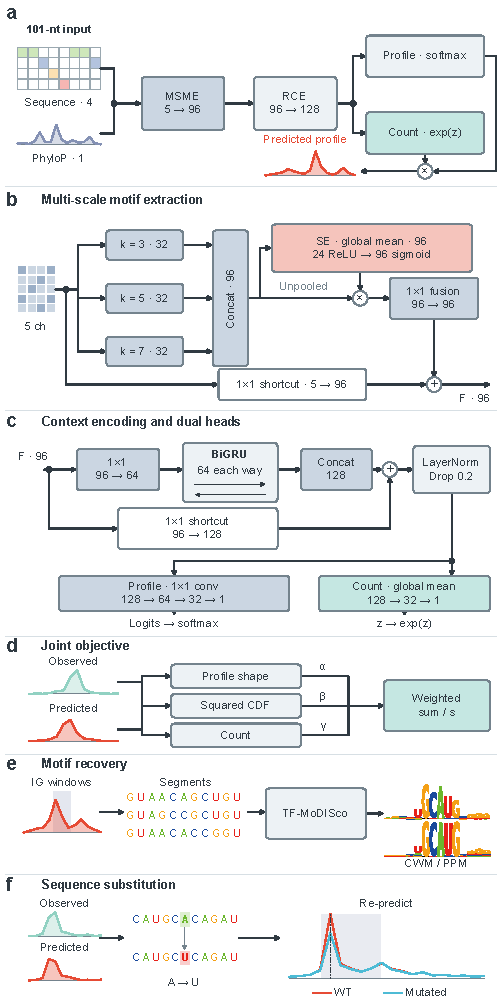
\includegraphics[width=85mm]{fig1.pdf}
\caption{CARBON architecture and prediction-based analyses. (\textbf{a}) Four sequence channels and aligned phyloP values form a 101-nt input. Profile logits are normalised by softmax and multiplied by $\exp(z)$, with $z$ from the count head. (\textbf{b}) Convolutions of widths 3, 5 and 7 produce 96 concatenated channels. SE weights rescale the unpooled features before fusion; an independent input projection supplies the residual. (\textbf{c}) A $96\rightarrow64$ projection feeds a bidirectional GRU with 64 units per direction. Its output is added to a $96\rightarrow128$ residual projection before layer normalisation and dropout. Three $1\times1$ convolutions ($128\rightarrow64\rightarrow32\rightarrow1$) form the profile head; global mean pooling and two linear maps ($128\rightarrow32\rightarrow1$) form the count head. (\textbf{d}) Profile-shape, squared-CDF and count terms jointly supervise prediction (Equation~\ref{eq:total_loss}). (\textbf{e}) IG-guided window selection and TF-MoDISco motif recovery lead to the Tomtom/CISBP-RNA comparison described in \supsect{S1.7}. (\textbf{f}) Sequence substitutions measure prediction sensitivity. Sequence fragments and curves illustrate the workflow; batch normalisation, hidden-layer activations and head dropout are specified in Methods and \supsect{S1.4}.}
\label{fig:figure1}
\end{figure}

\subsubsection{Multi-scale motif extraction and channel recalibration}\label{subsec:blocks}

The MSME applies three parallel one-dimensional convolutions with widths $k\in\{3,5,7\}$, each producing 32 channels. For output channel $d$,
\begin{equation}
T^{(k)}_{i,d}=b^{(k)}_d+
\sum_{j=-(k-1)/2}^{(k-1)/2}\sum_{c=1}^{5}
K^{(k)}_{j,c,d}X_{i+j,c}.
\label{eq:multiscale_convolution}
\end{equation}
Zero padding preserves length. Batch normalisation (BN) and GELU are applied in each branch:
$V^{(k)}=\operatorname{GELU}(\operatorname{BN}(T^{(k)}))$.
Concatenation gives $V_i=[V_i^{(3)};V_i^{(5)};V_i^{(7)}]\in\mathbb R^{96}$, retaining the common nucleotide coordinate.

A Squeeze-and-Excitation (SE) block \citep{hu2018senet} uses the pooled feature vector to calculate one gate per channel,
\begin{equation}
\begin{aligned}
m&=\frac1L\sum_{i=1}^{L}V_i,\\
a&=\sigma\!\left(W_2\operatorname{ReLU}(W_1m+b_1)+b_2\right).
\end{aligned}
\label{eq:se_gate}
\end{equation}
Here $\sigma(x)=(1+\exp(-x))^{-1}$, $W_1\in\mathbb R^{24\times96}$ and $W_2\in\mathbb R^{96\times24}$; the reduction ratio is 4. The same gate rescales every position's unpooled features. A pointwise fusion and an independent projected input shortcut \citep{he2016resnet} yield
\begin{equation}
F_i=W_f(a\odot V_i)+b_f+W_sX_i+b_s
\in\mathbb R^{96}.
\label{eq:motif_residual}
\end{equation}
The operator $\odot$ is elementwise multiplication; $W_f$ and $W_s$ map 96 and five channels, respectively, to 96. No activation follows the sum. SE thus supplies a global channel summary even in the NoGRU control.

\subsubsection{Recurrent context encoding}

The RCE first projects $F_i$ to $e_i=W_pF_i+b_p\in\mathbb R^{64}$ and applies a single bidirectional GRU \citep{cho2014rnnencoder,schuster1997brnn}. For one direction, with $h_0=0$ and 64 hidden units, the reset gate, update gate, candidate and state follow the PyTorch convention:
\begin{align}
r_i&=\sigma(W_{ir}e_i+b_{ir}+W_{hr}h_{i-1}+b_{hr}),
\label{eq:gru_reset}\\
g_i&=\sigma(W_{ig}e_i+b_{ig}+W_{hg}h_{i-1}+b_{hg}),
\label{eq:gru_update}\\
n_i&=\tanh\!\big(W_{in}e_i+b_{in}
\nonumber\\[-2pt]
&\hspace{18mm}+r_i\odot(W_{hn}h_{i-1}+b_{hn})\big),
\label{eq:gru_candidate}\\
h_i&=(1-g_i)\odot n_i+g_i\odot h_{i-1}.
\label{eq:gru_state}
\end{align}
Each $W_{i*}$ and $W_{h*}$ is $64\times64$. The reverse direction has independent parameters and a zero terminal state. Concatenating directional states and adding a $96\rightarrow128$ shortcut gives
\begin{equation}
v_i=[\overrightarrow h_i;\overleftarrow h_i]+W_rF_i+b_r
\in\mathbb R^{128}.
\label{eq:bidirectional_sum}
\end{equation}
Layer normalisation \citep{ba2016layernorm} operates across features at each position, followed by dropout:
\begin{equation}
\begin{aligned}
\mu_i&=\frac1{128}\sum_{d=1}^{128}v_{i,d},\\
\nu_i&=\frac1{128}\sum_{d=1}^{128}(v_{i,d}-\mu_i)^2,\\
u_i&=\mathcal D_{0.2}\!\left(
\eta\odot\frac{v_i-\mu_i}{\sqrt{\nu_i+10^{-5}}}+\xi\right).
\end{aligned}
\label{eq:recurrent_residual}
\end{equation}
The learned scale and offset are $\eta,\xi\in\mathbb R^{128}$; $\mathcal D_{0.2}$ denotes dropout with probability 0.2, disabled at inference. NoGRU removes the recurrent path and its input projection while retaining the shortcut, normalisation and dropout. CARBON uses GRU and SE context without multi-head self-attention; iDeepB uses a BiLSTM followed by multi-head attention \citep{liu2025ideepb}.

\subsubsection{Profile and total-count decoding}

The profile head transforms $u_i$ with pointwise layers of widths $128\rightarrow64\rightarrow32\rightarrow1$. With $q_i^{(0)}=u_i$, its two hidden layers and final logit are
\begin{equation}
\begin{aligned}
q^{(j)}&=\mathcal D_{0.2}\!\left[
\operatorname{GELU}\!\left(\operatorname{BN}(A_jq^{(j-1)}+a_j)\right)\right],\\
\ell_i&=w_3^\top q_i^{(2)}+a_3,\qquad j=1,2.
\end{aligned}
\label{eq:profile_head}
\end{equation}
The affine maps $A_j$ are $1\times1$ convolutions and preserve position. The count head pools across positions and uses a 32-unit hidden layer,
\begin{equation}
\begin{aligned}
\bar u&=\frac1L\sum_{i=1}^{L}u_i,\\
z&=w_c^\top\mathcal D_{0.2}\!\left[
\operatorname{GELU}(W_c\bar u+b_c)\right]+b_o,
\end{aligned}
\label{eq:count_head}
\end{equation}
where $W_c\in\mathbb R^{32\times128}$ and $w_c\in\mathbb R^{32}$. Profile--count factorisation separates spatial allocation from magnitude \citep{avsec2021bpnet}. For window $b$, the evaluated decoder is
\begin{equation}
p_{b,i}=\frac{\exp(\ell_{b,i})}{\sum_{j=1}^{L}\exp(\ell_{b,j})},
\qquad \hat y_{b,i}=p_{b,i}\exp(z_b).
\label{eq:dual_head_decode}
\end{equation}
Thus $\sum_i p_{b,i}=1$ and the reconstructed total is $\exp(z_b)$.

\subsubsection{Training objective}\label{subsec:loss}

CARBON jointly supervises allocation, spatial displacement and total signal. For batch size $B$, observed signal $y_{b,i}$ and total $S_b=\sum_i y_{b,i}$, define
\begin{align}
\mathcal L_{\rm shape}
&=-\frac1B\sum_{b=1}^{B}\sum_{i=1}^{L}y_{b,i}\log p_{b,i},
\label{eq:shape_loss}\\
\mathcal L_{\rm CDF}
&=\frac1{BL}\sum_{b=1}^{B}\sum_{i=1}^{L}
\left(\sum_{j\leq i}p_{b,j}-\sum_{j\leq i}\tilde y_{b,j}\right)^2,
\label{eq:cdf_loss}\\
\mathcal L_{\rm count}
&=\frac1B\sum_{b=1}^{B}\left[z_b-\log(S_b+1)\right]^2,
\label{eq:main_count_loss}
\end{align}
with $\tilde y_{b,i}=y_{b,i}/(S_b+\varepsilon)$ and $\varepsilon=10^{-6}$. The shape term is count-weighted cross-entropy: high-total windows contribute more strongly. The squared CDF term penalises displacement of predicted mass; it is distinct from the transport-cost definition of Earth Mover's Distance \citep{rubner2000emd} and from one-dimensional Wasserstein-1. Its separate contribution to assay-shift tolerance was not tested. For zero-count windows, the shape term vanishes and $\tilde{\mathbf y}_b=\mathbf0$; the other terms remain defined.

The combined objective is
\begin{equation}
\mathcal L=\frac1s
\left(\alpha\mathcal L_{\rm shape}+
\beta\mathcal L_{\rm CDF}+\gamma\mathcal L_{\rm count}\right),
\label{eq:total_loss}
\end{equation}
where $s=1$ and the selected weights are $\alpha=1.4194219$, $\beta=0.5402181$ and $\gamma=1.7983396$. An eight-parameter Optuna search selected these weights jointly with optimisation settings \citep{akiba2019optuna}. The reconstruction in Equation~\ref{eq:dual_head_decode} uses $\exp(z)$ although the target is $\log(S+1)$, giving total $S+1$ at an exact fit. Replacing the multiplier by $\max(\exp(z)-1,0)$ in the same chromosome-8/15 forward passes changed mean pooled PCC and Spearman by $6.5\times10^{-5}$ and $3.7\times10^{-5}$, respectively. We retain the evaluated convention (\supsect{S1.5,S1.11}; Data S14).

\subsection{Implementation details}\label{sec:impl}

CARBON was implemented in PyTorch and fitted with AdamW, batch size 256, initial learning rate $7.851013\times10^{-4}$, weight decay $1.143421\times10^{-4}$ and gradient-clipping norm 2. The 65-trial, five-task search selected the configuration by mean validation PCC. Final benchmark runs used seed 0 and at most 100 epochs. The training loop halved the learning rate after five epochs without improvement in mean validation loss and stopped below $10^{-7}$. A separate rule saved checkpoints by validation Peak AP and stopped after nine non-improving epochs. These validation-loop summaries differ from the task-wide offline evaluation metrics (\supsect{S1.4}). The benchmark has one fit per task/arm; \supsect{S1.16} reports the limited two-task, three-seed sensitivity analysis.

The native allocation experiment instead used matched architectural fits with seeds 11/23/47 and validation-PCC selection. External-preference and natural-variant analyses used existing Full/Sequence checkpoints without retraining; matched training histories for those two families have not been established. Full-flat and Full-permuted alter conservation input within the same Full checkpoint. They are input perturbations, whereas Sequence is a separately fitted model.

Training jobs were dispatched across an NVIDIA L40 and three Quadro RTX 6000 GPUs. Bulk conservation inference used one L40, batch size 256 and four CPU threads. Because hardware and concurrent load were not matched across historical jobs, elapsed times describe execution rather than hardware-normalised efficiency (\suptab{S3}). Software versions, selected input/checkpoint identities and availability are detailed in \supsect{S1.9,S1.10}.

\subsection{Evaluation protocol}\label{subsec:metrics}

\subsubsection{Profile prediction and component comparisons}

PCC and Spearman correlate concatenated observed and predicted positions within each task. Reported benchmark means weight tasks equally; they are not means of within-window correlations. Signal AUROC and average precision (AP) use the task-wide observed median as a strict positive threshold. Peak AUROC/AP score bases in contiguous non-zero segments with maximum signal at least two or segment sum at least two. The historical implementation detects these segments in the flattened vector without resetting at window boundaries. Correlation and ranking metrics therefore measure distinct aspects of prediction \citep{davis2006prroc,saito2015precision}; exact rules are in \supsect{S1.1}.

Five CARBON ablations use this common evaluator. They remove the conservation channel, recurrent path, multi-scale branches or SE gate, or replace the combined objective with a Poisson reconstruction loss,
\begin{equation}
\mathcal L_{\rm rec}=\frac1{BL}\sum_{b=1}^{B}\sum_{i=1}^{L}
\left[\hat y_{b,i}-y_{b,i}\log\!\left(\max\{\hat y_{b,i},10^{-20}\}\right)\right],
\label{eq:reconstruction_loss}
\end{equation}
where $\hat y_{b,i}=p_{b,i}\exp(z_b)$ as in Equation~\ref{eq:dual_head_decode}. This objective replaces all three weighted terms in Equation~\ref{eq:total_loss}; the lower bound stabilises only the logarithm. Architectural removals also change feature width or parameter count. Paired task tests are exploratory and do not estimate benchmark-wide training uncertainty (\supsect{S1.4,S1.5,S1.9}).

Historical iDeepB and RBPNet scores are reported with their original output and evaluation definitions. CARBON and iDeepB produce count-like outputs, whereas the evaluated RBPNet treatment profile has unit sum per window. RBPNet also differs in its local-maximum peak rule, tied-rank handling and ambiguous-base filtering. Common task names therefore establish neither matched windows nor matched estimands. These scores describe the retained implementations and cannot establish a fair cross-method ranking (\supsect{S1.3}).

\subsubsection{Motif recovery and conservation diagnostics}\label{subsec:interp}

Integrated Gradients (IG) \citep{sundararajan2017integrated} and within-task TF-MoDISco clustering \citep{shrikumar2018tfmodisco} identify attributed sequence patterns. Tomtom compares recovered patterns with cognate human CISBP-RNA motifs \citep{ray2013compendium,gupta2007tomtom,bailey2015meme}; exact RBP names and motif IDs link each comparison to direct-experimental, compiled, homology-inferred or JPLE-inferred provenance. The original $p$ and $q$ values are retained. An additional search compares all 485 stored motifs from 219 tasks with all 1,583 matrices in the official ATtRACT snapshot \citep{giudice2016attract}. Each query is searched against the full target family before same-RBP filtering or post hoc display selection (\supsect{S1.19}; Data S24).

The positive pattern-0 overview uses maximal-information 9-nt crops, Euclidean distance between row-normalised position-probability matrices and average-linkage clustering. The resulting tree organises sequence patterns, rather than evolutionary relatedness. Figure~3b's six illustrative ATtRACT pairs require human, unmutated, same-RBP references of width $\leq10$ nt, $q<0.01$ and mean query information content $\geq0.3$ bits in both matched and displayed intervals. Five prioritise $q$ and one information content. The complete search and non-significant results accompany the display.

\textit{In silico} mutagenesis substitutes bases in representative cores to assess fitted prediction sensitivity \citep{zhou2015deepsea}. Attribution plausibility alone does not validate a mechanism \citep{adebayo2018sanity}, and one-hot gradients can contain off-simplex noise \citep{majdandzic2023gradient}. The unresolved final IG target/baseline/steps, exact substitution and checkpoint linkage for the three historical examples are specified in \supsect{S1.7}. Data S24 separately retains six CISBP examples with direct-experimental references selected by task/reference-ID order, independently of comparison scores.

\paragraph{Conservation diagnostics.}\label{subsec:perturb_methods}
Trained-model stratification, fixed-checkpoint positional perturbations and factorial substitutions examine different relationships between conservation, observed signal and model response. The localization cohort contains 2,079,810 eligible records; bulk perturbation uses 706,642 windows; the factorial study uses 1,120 windows. Correlations are paired within windows and aggregated at their specified task/RBP levels, separately from pooled benchmark correlations. These analyses assess association and model reliance; a larger sequence response is not itself evidence of greater biological accuracy (\supsect{S1.8,S1.11--S1.14}; \supfig{S3,S5--S13}).

\subsubsection{Native repeated-core allocation}\label{subsec:allocation_methods}

We evaluated allocation between repeated PTBP1 CTCT cores in native 101-nt windows. Full, NoGRU and Local+pos all retain sequence, PhyloP and the global SE gate. Local+pos adds explicit feature-by-position interactions and nearly matches Full's capacity. Each arm was fitted on chromosomes 3--7, 10--14 and 17--22, with validation chromosomes 2/9/16 and seeds 11/23/47. Query chromosomes 1/X/Y were held out from these fits within a development-informed study.

The first two eligible CTCT occurrences separated by at least 12 nt define inclusive $\pm5$-nt supports $\mathcal S_1,\mathcal S_2$. A fixed input-identity hash chooses a representative among overlapping windows. Eligible pairs map uniquely to a gene, have positive whole-window signal and input-control totals, and meet the non-negative residual criteria below. For eCLIP/input-control support sums $y_j,b_j$ and whole-window totals $Y,C$, the target and three-seed predicted share are
\begin{equation}
\begin{aligned}
r_j&=y_j-\frac{Y}{C}b_j,\qquad
q_1=\frac{r_1}{r_1+r_2},\\
\bar p_i^{(m)}&=\frac13\sum_{s\in\{11,23,47\}}p_i^{(m,s)},\\
p_1^{(m)}&=
\frac{\sum_{i\in\mathcal S_1}\bar p_i^{(m)}}
{\sum_{i\in\mathcal S_1\cup\mathcal S_2}\bar p_i^{(m)}}.
\end{aligned}
\label{eq:allocation_readout}
\end{equation}
We require $r_1,r_2\geq0$ and $r_1+r_2>0$; negative residuals are excluded rather than clipped. Profiles are averaged before conditioning, rather than averaging seed-specific shares. The input-adjusted $q_1$ is an allocation target, not a calibrated physical-binding probability.

Let $G_c$ denote eligible genes in cell $c$ and $\mathcal P_{cg}$ the pairs for gene $g$. The primary mean squared error (MSE) is
\begin{equation}
\begin{aligned}
E_m&=\frac12\sum_{c\in\{K562,HepG2\}}\frac1{|G_c|}
\sum_{g\in G_c}\frac1{|\mathcal P_{cg}|}\\[-2pt]
&\hspace{15mm}\times\sum_{k\in\mathcal P_{cg}}
\left(p_{1,k}^{(m)}-q_{1,k}\right)^2 .
\end{aligned}
\label{eq:allocation_estimator}
\end{equation}
Genes receive equal weight within each cell, then the two cells are weighted equally. A joint bootstrap of real gene IDs preserves model pairing and shared-gene cross-cell dependence. We used 10,000 replicates and Bonferroni-adjusted intervals for the two-comparison family Full-minus-Local+pos and Local+pos-minus-NoGRU. The complete cohort, seed contrasts and post hoc example-selection rule are in \supsect{S1.17} and Data S22. Figure~4c instead displays raw support-conditioned observed signal $y_1/(y_1+y_2)$ and predicted shares before row averaging; these visual summaries differ from the input-adjusted endpoint.

\subsubsection{External sequence-preference evaluation}\label{subsec:order_methods}

The intersection of human RNAcompete measurements and Full/Sequence checkpoint availability yielded 28 proteins. Excluding HNRNPK, PTBP1 and RBFOX2, which had been explored previously, defines the 25-protein group: 36 tasks and 34 measured RNAcompete columns. All available matching measurements are retained. Seven-mer Z scores are converted to $Z_5(w)$ by averaging every overlapping occurrence of five-mer $w$ in the available seven-mer matrix \citep{ray2013compendium}. This is an occurrence-weighted preference proxy, rather than a direct affinity measurement of the edited native sequence.

For each task, 16 hash-selected eligible chromosome-8/15 windows supply fixed 101-nt backgrounds. Positions 49--53 (1-based) are replaced with every one of the $4^5=1,024$ words. Full retains the original PhyloP vector; Sequence has no conservation channel. Replacement-minus-native count-head outputs are averaged across backgrounds. For two words in background $s$,
\begin{equation}
\Delta_{w\to w'}(s,\phi)
=z(s^{(w')},\phi)-z(s^{(w)},\phi),
\label{eq:word_response}
\end{equation}
where $s^{(w)}$ denotes replacement by $w$. Positive values favour the word on the right of the arrow.

The primary endpoint is Spearman correlation over all 1,024 words. The secondary endpoint evaluates all 15,240 word pairs within the 56 exact base-count groups, excluding experimental ties and scoring exact prediction ties as 0.5. Metrics are calculated per task/assay, averaged within protein/cell and then equally across a protein's available cells. Paired 95\% percentile intervals use 10,000 protein bootstrap resamples. Native Frequency counts every overlapping five-mer in up to 1,024 hash-selected native windows per task. Adjacent-swap illustrations use differences of these existing outputs; contexts and word pairs are computational units, not additional biological replicates. Full/Sequence training histories are not verified as matched, and the native backgrounds had already been evaluated in the benchmark. RNAcompete supplies the independent measurement (\supsect{S1.18}; Data S23).

\subsubsection{Natural variants and linked biological annotations}\label{subsec:variant_methods}

We compared allele-paired predictions with published BEAPR ASB calls \citep{yang2019asb}. The previously analysed chromosome-8/15 subset contains 396 significant ASB events at 287 exact GRCh38 REF/ALT variants across 85 RBPs. Each allele pair receives the same original reference PhyloP vector. For source-preferred allele $s_e^+$ and other allele $s_e^-$, direction credit is
\begin{equation}
\begin{aligned}
d_e&=z(s_e^+,\phi_e)-z(s_e^-,\phi_e),\\
a_e&=\mathbf1[d_e>\tau]
+\tfrac12\mathbf1[|d_e|\leq\tau],
\qquad \tau=10^{-7}.
\end{aligned}
\label{eq:allele_direction}
\end{equation}
Here $\mathbf1[\cdot]$ is an indicator. We compare Full, Sequence, fixed-checkpoint flat/permuted input and a constant reference-allele preference rule. The permuted-input response is averaged across three permutations before direction scoring. With eligible RBPs $\mathcal R$, their tasks $\mathcal T_r$ and task events $\mathcal E_t$, accuracy is
\begin{equation}
A=\frac1{|\mathcal R|}\sum_{r\in\mathcal R}
\frac1{|\mathcal T_r|}\sum_{t\in\mathcal T_r}
\frac1{|\mathcal E_t|}\sum_{e\in\mathcal E_t}a_e.
\label{eq:allele_accuracy}
\end{equation}
Events are averaged within tasks, tasks within RBP and RBPs equally. Aggregate accuracy and paired-contrast intervals use 2,000 positive-exponential multiplier draws over RNA-region and RBP clusters. Descriptive conservation associations adjust for task, local sequence, composition, mutation class, strand, sequencing depth and reference preference; their first-order clustered score intervals are accompanied by weighted-refit checks (\supsect{S1.20}; Data S25). All events were development-exposed; the ASB-positive design evaluates direction conditional on a positive call, rather than detection of ASB.

For biological context, we matched the complete existing variant set to exact GRCh38 alleles in ClinVar, public TCGA/GDC and population records, preserving unavailable frequencies. Exact mutagenesis-primer and allele-orientation matching links all eleven published two-allele reporter loci to 24 associated ASB events and 66 source biological measurements. Reporter expression/splicing and predicted binding remain distinct endpoints. All matches, failed model directions and post hoc selection records are retained (\supsect{S1.21,S1.22}; Data S26--S27).

\paragraph{Cross-cell evaluation.}
K562--HepG2 transfer uses 70 RBP symbols present in both directions, giving 140 directional records. The peak-overlap analysis uses the 64-symbol subset with available overlap measurements, with two directions averaged within symbol before tertile grouping. Repeated directions and shared proteins preclude treating every record as an independent biological observation (\supsect{S1.6}).

\section{Results}\label{sec:results}

\subsection{CARBON predicts base-resolution profiles across 150 RBPs}\label{subsec:benchmark}

Across 222 tasks, CARBON achieved mean task-pooled PCC 0.3092 and Spearman 0.4226 (\figrefwhole{fig:figure2}; \suptab{S1}). Task variation is visible in the complete score ring, six-metric distributions and paired comparisons (\figpanelref{fig:figure2}{a--g}). The FMR1 example connects these summaries to local profile shape (\figpanelref{fig:figure2}{h}); its downward tracks show inverted pooled eCLIP and input-control signal.

The historical summaries place CARBON above the retained iDeepB and RBPNet implementations in PCC for 220/222 tasks and in Spearman for all tasks. These values are descriptive: the evaluated outputs, peak definitions, tie handling and potentially eligible windows differ between implementations (Section~\ref{subsec:metrics}). The FMR1 locus correlations also lack complete raw-array linkage. We therefore assess component contributions with a common within-CARBON evaluator and examine allocation and sequence preferences through their specifically defined endpoints.

\subsection{Recurrent context and conservation improve complementary aspects of prediction}\label{subsec:ablation}

Among five component ablations, removing the recurrent path caused the largest reduction: mean Spearman declined by 0.1064 and PCC by 0.0859, with lower values in 222/222 and 221/222 tasks, respectively (\suptab{S2}; \supfig{S1}). Context encoding is consequently the most influential tested architectural component. Because recurrent removal also reduces capacity, the native allocation analysis below includes a near-capacity alternative.

Removing conservation reduced mean Spearman by 0.0234 and PCC by 0.0227; scores declined in 219 and 213 tasks, respectively. The four discrimination metrics also fell by 0.015--0.018. Conservation therefore improves prediction relative to sequence alone under the fixed CARBON architecture and objective. Multi-scale convolution and SE removal produced smaller mean Spearman decreases of 0.0016 and 0.0012, placing their contribution in refinement of the complete model.

The loss ablation exposes a different trade-off. The Poisson reconstruction objective increased mean PCC by 0.0133, but lowered mean Spearman by 0.0130 and worsened discrimination metrics in 97.3--97.7\% of tasks. Only 82 tasks improved in PCC; the median paired change was $-0.0039$ (IQR $[-0.0116,0.0111]$). A few large improvements drove the positive PCC mean. The combined objective gives a more balanced result across agreement and ranking, although this joint comparison does not isolate its individual loss terms. We next examine the learned sequence features before testing the spatial role of context directly.

\begin{figure}[!tbp]
\centering
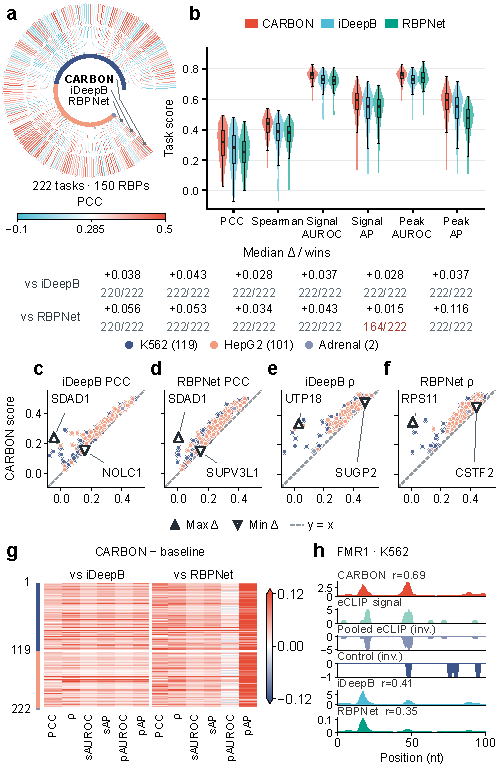
\includegraphics[width=85mm]{fig2.pdf}
\caption{Profile prediction across the benchmark and archived cross-model scores. \textbf{a}, PCCs for all 222 tasks, displayed with one shared light-blue--white--red power map ($\gamma=0.65$) over $[-0.1,0.5]$, with white at the pooled median of all 666 scores (0.285). The nonlinear contrast changes the display only; ticks retain PCC units. The wider outer ring highlights model identity and does not encode a score. \textbf{b}, Six-metric distributions, paired median differences and strict wins. Boxes show medians and interquartile ranges; whiskers extend to 1.5 IQR. \textbf{c--f}, Paired PCC (c,d) and Spearman (e,f) scores, with CARBON on y and the named comparator on x; triangles mark the largest and smallest gains. \textbf{g}, CARBON-minus-comparator differences on a shared zero-white scale with $\pm0.12$ limits; 195 values saturate. \textbf{h}, FMR1 profile predictions with inverted pooled eCLIP and control tracks, which are not replicates. Historical locus correlations cannot be fully reconstructed from identified raw arrays. The three implementations used unmatched output scales, scoring procedures and potentially different windows; these scores do not establish a fair method ranking. Definitions and sources: S1.3/S1.15 and Data S1/S3/S20.}
\label{fig:figure2}
\end{figure}

\subsection{Learned patterns recover cognate preferences with variable specificity}\label{subsec:motif}

Positive pattern-0 motifs from 219 tasks span all 150 RBP symbols (\figpanelref{fig:figure3}{a}). Their maximal-information 9-nt crops form a sequence-similarity overview, with functional and RNA-binding-domain annotations providing biological context. The complete names and enlarged atlas are retained in \supfig{S21}. This overview maps the model's learned preferences; reference matching supplies a separate test of cognate agreement.

The original CISBP-RNA set contains 193 comparisons from 80 task--pattern pairs, 45 tasks and 31 RBPs. Of 126 comparisons to direct-experimental references covering 27 RBPs, 45 pass the original $q<0.05$ threshold and represent 13 RBPs. Compiled, inferred and non-significant comparisons remain in Data S24. This source distinction separates resemblance to a measured preference from resemblance to a database inference.

Searching all 485 stored motifs against all 1,583 official ATtRACT matrices broadened the reference comparison \citep{giudice2016attract}. The exact same-RBP, human, unmutated subset contains 1,626 comparisons; 234 have $q<0.05$, covering 32 tasks and 22 RBPs. The database combines heterogeneous assay sources, and several low-$q$ references are homopolymers. Statistical motif agreement can thus capture low-complexity preference without establishing fine RBP specificity.

The six pairs in \figpanelref{fig:figure3}{b} illustrate this agreement on a common information-content scale. Their post hoc selection adds reference-width and query-information criteria after the complete search; $q$ values retain each query's full target family. The complete results include a significant but low-information PCBP1 query that fails the display criteria (\supsect{S1.19}; Data S24). The selected pairs demonstrate interpretable examples rather than the frequency of successful matching across the atlas.

Attribution and substitutions connect a recognised pattern to prediction sensitivity (\figpanelref{fig:figure3}{c}). PUM2 K562 matches a direct-experimental CISBP reference with $p=4.53\times10^{-5}$ and $q=0.0271$. The two HNRNPA1 examples respond to substitution even though their original cognate matches are non-significant ($q\approx0.312$ and 0.305). Pattern resemblance and fitted sensitivity are therefore complementary observations. Their mechanistic scope is limited by the historical attribution settings described in \supsect{S1.7}, motivating comparisons with measured allocation and external sequence preferences.

\begin{figure}[!tbp]
\centering
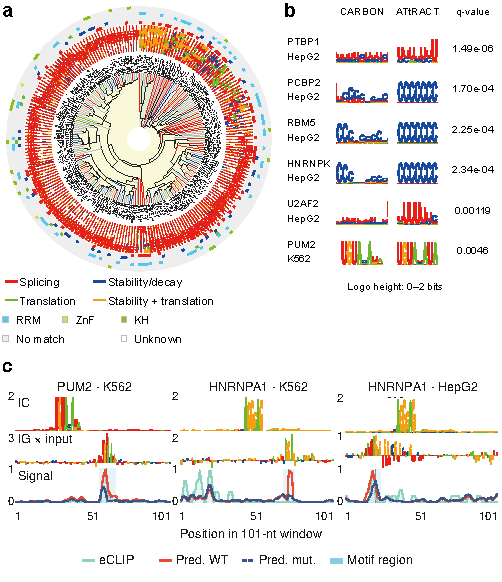
\includegraphics[width=85mm]{fig3.pdf}
\caption{Learned motif landscape, reference agreement and sequence sensitivity. \textbf{a}, All 219 positive pattern-0 motifs from 150 RBPs, with the complete name set, Euclidean PPM/average-linkage topology and leaf order. Terminal-branch colours indicate function; the six annotation rings show splicing, stability/decay, translation, RRM, ZnF and KH. Pastel sectors are six cuts of this same tree for visual orientation, not biological classes. Grey indicates no annotation-rule match. Figure~S21 provides an enlarged named atlas. \textbf{b}, Aligned CARBON and official ATtRACT logos on a common 0--2-bit scale. Six illustrative pairs were selected post hoc from positive pattern-0 queries and human, unmutated same-RBP references of width $\leq10$ nt, requiring $q<0.01$ and mean matched/displayed query information content $\geq0.3$ bits. Five prioritise $q$ and the sixth information content. All 485 queries were searched against all 1,583 references before selection; $q$ is adjusted within each query's complete target family. Data S24 includes the full results, low-information queries and non-significant matches. \textbf{c}, Three PUM2/HNRNPA1 examples linking the pattern logo, attribution and substitution sensitivity. Pattern and native-window coordinates differ; shading marks motif regions and dashes mark perturbation positions. Their CISBP statistics and interpretation limits are distinct from the ATtRACT analysis in b (S1.7/S1.19). A/C/G/U are green/blue/orange/red throughout.}
\label{fig:figure3}
\end{figure}

\subsection{Context processing improves allocation between repeated short cores}\label{subsec:allocation}\label{subsec:conservation}

Repeated cores provide a spatial test that motif presence alone cannot solve: two occurrences in one window can receive very different observed signal. The PTBP1 cohort contains 1,851 eligible CTCT pairs from 659 genes and 865 cell--gene units across K562 and HepG2 (\figpanelref{fig:figure4}{c}). The primary endpoint compares predicted support shares with input-adjusted local signal, weighting genes equally within each cell and cells equally.

Full achieved MSE 0.079884, compared with 0.115116 for NoGRU and 0.112084 for Local+pos. Local+pos has explicit feature-by-position interactions and 100,871 parameters, close to Full's 100,826. Relative to Local+pos, Full reduced MSE by 28.73\% ($\Delta$MSE $-0.032200$; two-comparison Bonferroni-adjusted 95\% interval $-0.039564$ to $-0.024750$). All three seed contrasts had the same sign. Contextual architecture therefore improves the measured allocation decision beyond the tested local, position-aware alternative, constraining a simple parameter-count explanation.

ZMYM4 illustrates how that decision arises (\figpanelref{fig:figure4}{a}). Its centred seven-mers are both TTCTCTT, yet their supports contain 28 and two units of eCLIP signal. Full assigns 93.0\% of its combined support mass to the first occurrence, close to the observed 93.3\%; NoGRU and Local+pos assign 49.7\% and 48.4\%. Differences outside the seven-mers, including flanking sequence and PhyloP, remain available to the models. The OCRL example retains the converse outcome: Full favours the wrong support while both controls are closer to the observation (\figpanelref{fig:figure4}{b}). The post hoc rule yielding ZMYM4, all eight qualifying cases and the OCRL failure are retained in \supfig{S19}.

The full atlas places measured and predicted profiles side by side for every cell--gene row. Shared support-1 share strips and cell-wise scatterplots expose both agreement and misallocation, without selecting successful rows. ZMYM4's row averages two pairs; its detailed panel shows one. These raw-share displays contextualise the input-adjusted MSE endpoint; the complete adjusted error-difference map, including larger Full errors, remains in \supfig{S20}.

The supporting HNRNPK comparison also favours Full over NoGRU across 1,418 pairs and 527 genes ($\Delta$MSE $-0.025929$; Bonferroni-12 interval $-0.034304$ to $-0.017086$), but lacks the near-capacity control (\supsect{S1.17}; Data S22). All allocation arms retain conservation and global SE. The result establishes an architectural allocation advantage, rather than a conservation-specific effect.

\begin{figure}[!tbp]
\centering
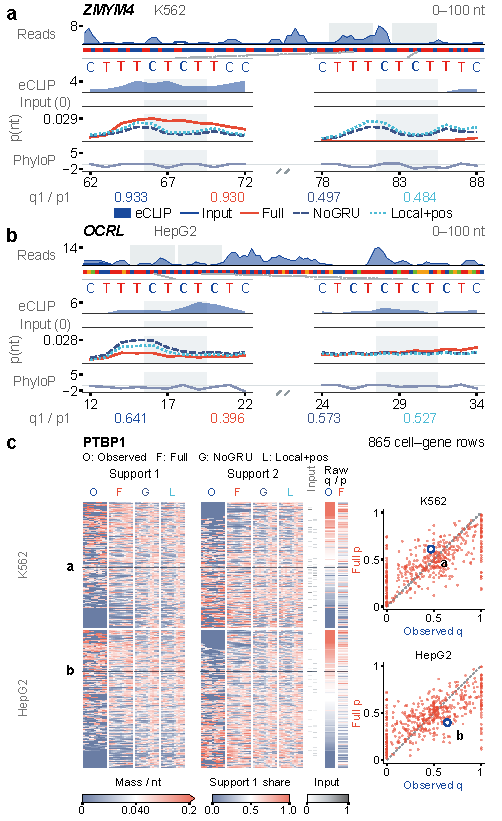
\includegraphics[width=85mm]{fig4.pdf}
\caption{Allocation between repeated short cores in native RNA context. \textbf{a,b}, ZMYM4 and the OCRL failure, showing native 101-nt signal and two inclusive 11-nt supports. ZMYM4 has identical centred seven-mers; OCRL shares CTCT only. Coordinates are zero-based, and observed eCLIP and size-matched input-control tracks are navy. The numeric row reports the adjusted observed share $q_1$ and three-seed Full/NoGRU/Local+pos shares $p_1$. \textbf{c}, All 1,851 pairs, 659 genes and 865 cell--gene rows. Observed and model profiles are jointly conditioned on the 22 support positions before row averaging and share one mass-per-nucleotide colour scale. Adjacent observed/Full support-1 share strips use one 0--1 scale; input is displayed separately in grey. The right-hand scatter compares observed raw share with Full share for all 412 K562 and 453 HepG2 rows, with an identity line for agreement. Marks a/b identify the corresponding gene rows: ZMYM4 averages two pairs, while a shows one pair. Raw shares in c differ from the input-adjusted targets in a,b. The adjusted MSE reduction of 28.73\% versus Local+pos is evaluated separately in S1.17/Figure~S20. All three model arms retain conservation input. Complete cases, unsuccessful allocations and source arrays are provided in S19/S20 and Data S22.}
\label{fig:figure4}
\end{figure}

\subsection{Sequence-order responses agree with external word preferences}\label{subsec:external_preference}\label{subsec:perturb_results}

We next tested whether predicted sequence responses agree with independently measured binding preferences. Across 25 proteins, the primary all-word RNAcompete Spearman was 0.25744 for Full, 0.26931 for Sequence and 0.11126 for Native Frequency (\figpanelref{fig:figure5}{a}). Full exceeded Frequency by 0.14619 (95\% paired-protein bootstrap interval 0.03802--0.24800). Thus the learned response landscape tracks external word preferences beyond the abundance of those words in native windows.

Holding nucleotide composition constant asks a sharper question about order. Across all eligible equal-base-count word pairs, mean concordance was 56.62\% for Full, 57.31\% for Sequence and 52.84\% for Frequency. Full exceeded Frequency in 19/25 proteins, with mean difference 3.78 percentage points (95\% interval 0.90--6.73). Figure~5a retains every Full/Frequency pair and paired difference for both endpoints; \supfig{S31} retains all three arms. Both learned models improve on Frequency in mean agreement, while Sequence has the higher mean on both endpoints. These results support learned arrangement-dependent preferences without establishing a general Full--Sequence advantage.

The complete QKI landscape makes the order comparison explicit (\figpanelref{fig:figure5}{b}). It retains all 30 A$_2$C$_2$U words and 48 adjacent exchanges of different bases. Literal inversion rank determines the base geometry, while height encodes RNAcompete $Z_5$. Of 48 exchanges oriented towards greater external preference, Full and Sequence predict positive mean contrasts for 31 and 30, respectively. The three highlighted exchanges to CUAAC increase $Z_5$ from 0.5013 (UCAAC), 0.4595 (CAUAC) and 0.5507 (CUACA) to 2.6120. Full predicts positive changes in all 32 computational backgrounds for each; Sequence agrees in 32/32, 31/32 and 31/32. Both models' mean responses share a colour scale, and the complete individual response matrices remain in \supfig{S28b}. This previously explored landscape retains weak and adverse exchanges; its geometry is sequence topology, rather than a learned embedding or fitness surface.

HNRNPA1 provides a complementary comparison where preference opposes native abundance (\supfig{S28c}). UGAGG$\to$UAGGG reduces mean occurrence count from 244 to 143 while increasing RNAcompete-derived $Z_5$ from 1.32 to 6.37. Full and Sequence give mean changes $+0.04178$ and $+0.03630$, positive in 27/32 and 24/32 backgrounds. Both models therefore favour the externally preferred arrangement despite its lower abundance.

Full keeps reference PhyloP fixed throughout each replacement pair. The word analysis evaluates the sequence response against an external assay, not the effect of an edited native transcript or a mutant conservation score. Complete word landscapes, the separate frozen external-first selected-edit atlas and all 1,152 model/background responses remain in \supfig{S15--S18,S24,S26} and Data S23. These records retain unavailable cells, the weak TIA1 response, adverse candidates and assay-specific negative controls.

\begin{figure*}[p]
\centering
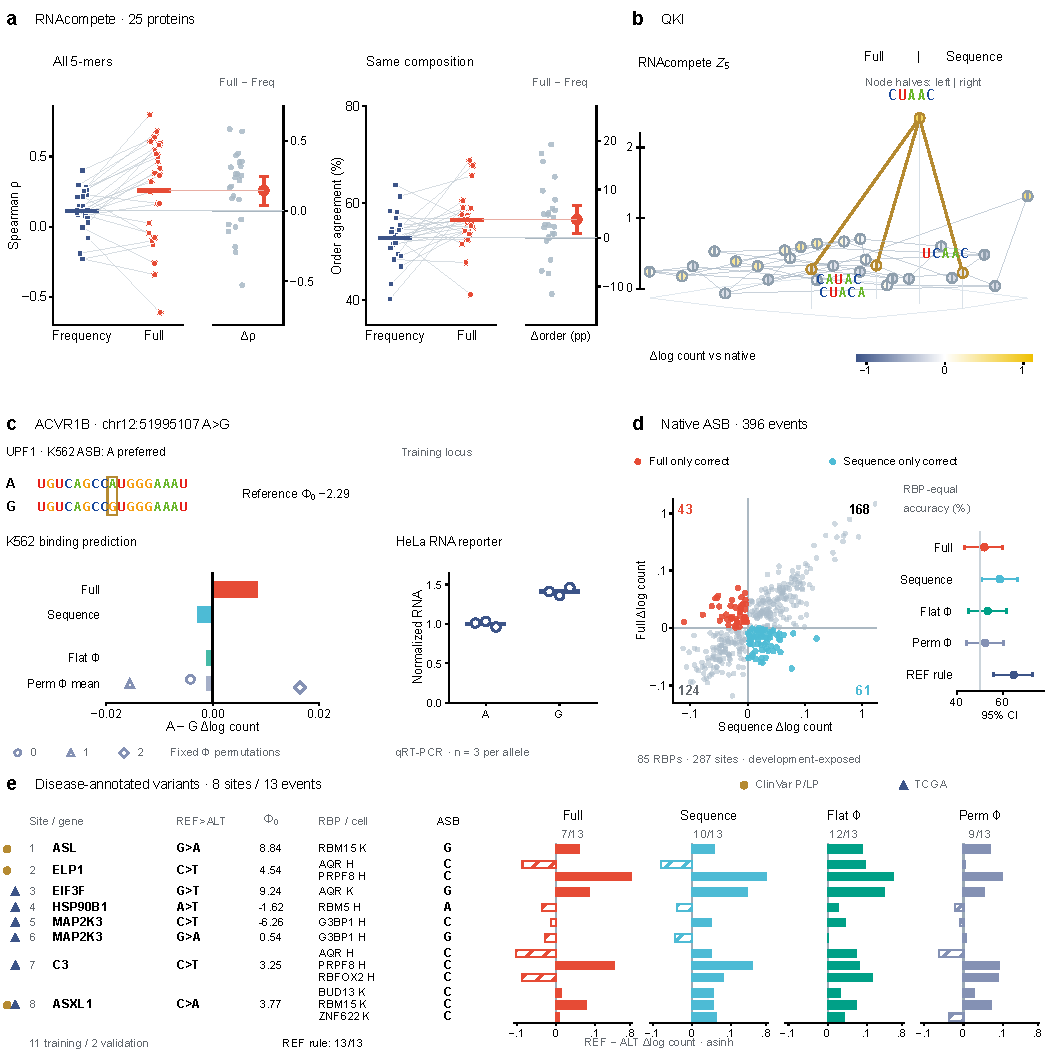
\includegraphics[width=178mm]{fig5.pdf}
\caption{External sequence preferences and source-resolved natural variants. \textbf{a}, All 25 proteins' paired Full/Frequency scores and differences for primary all-word Spearman and secondary composition-matched concordance. Adjacent difference axes share the absolute axes' units and spans, offset to the Frequency means. In the adjacent difference axes, red points and interval bars give frozen paired-protein means and 95\% bootstrap intervals; grey points are individual protein differences. The mean Full-minus-Frequency differences are $+0.146$ (95\% CI $+0.038$ to $+0.248$) for Spearman and $+3.78$ percentage points ($+0.90$ to $+6.73$) for composition-matched concordance. Complete Sequence controls remain in Figure~S31. \textbf{b}, All 30 QKI A$_2$C$_2$U words and 48 adjacent exchanges. Height encodes RNAcompete $Z_5$; node halves encode Full/Sequence mean responses across 32 computational backgrounds on a shared asinh colour scale. Gold marks three CUAAC-neighbour edges. \textbf{c}, Exact ACVR1B A$>$G, source UPF1 preference for A (ASB FDR 0.0446), seven saved model/control responses and published HeLa RNA reporter measurements from \citet{yang2019asb}. Hollow shapes identify three fixed-input permutations, not uncertainty or biological replicates. Reporter points are three biological measurements per allele with mean ticks; RNA abundance and predicted K562 binding are distinct endpoints. This is a post hoc training-locus illustration. \textbf{d}, All 396 exposed ASB-positive events, with source-preferred-minus-other responses and five-arm RBP-equal accuracy/95\% intervals. Red/cyan identify Full-only/Sequence-only direction agreement. \textbf{e}, All eight ClinVar P/LP and/or TCGA-overlap sites, 13 events and four-arm REF-minus-ALT responses. Filled/open hatched bars favour REF/ALT; every source label favours REF. Agreement counts are 7/10/12/9 for Full/Sequence/flat/permuted input; the constant-REF rule gives 13/13. H/K denote HepG2/K562. These events include 11 training and two validation observations, with no strict-test events. Disease annotations do not establish binding truth or clinical causality. Both axes in d and all four effect axes in e share asinh width 0.02 within their panel; ticks retain original log-count units. The reference conservation input is fixed across each allele pair. Exact site identities: Figure~S32. Methods S1.18/S1.20--S1.22; Data S23/S25--S27.}
\label{fig:figure5}
\end{figure*}

\subsection{Exact reporter-site matching links allele judgments to regulatory measurements}\label{subsec:reporter_variants}

Natural variants connect sequence-order decisions to experimentally observed allele preferences. We first established exact identity between all eleven two-allele reporter loci in \citet{yang2019asb} and the saved 101-nt inputs, using mutagenesis primers and allele orientation. This yields 24 ASB events and all 66 original biological measurements (\supfig{S29,S30}; Data S27). These are previously exposed loci: 21 events fall on training chromosomes and three on validation chromosomes. Their role is to connect predictions and regulatory measurements at the same variant.

At ACVR1B chr12:51,995,107 A$>$G, source K562 UPF1 binding favours A (\figpanelref{fig:figure5}{c}). Full predicts A-minus-G log-count change $+0.008365$, whereas Sequence predicts $-0.002801$. Flat-input and permutation-mean controls are also negative, although one of three individual permutations is positive. The published HeLa reporter has mean mCherry/eYFP ratios 1.00 for A and 1.41 for G, with three biological measurements per allele. The preferred-binding allele thus accompanies lower reporter RNA abundance, consistent with a possible UPF1-related turnover hypothesis. The binding prediction does not estimate that expression ratio or establish UPF1 mediation.

The GWAS-associated CERS2 rs267738 provides a different biological connection (\supfig{S29,S30}). Its genomic T$>$G is RNA A$>$C. Full and Sequence both favour the GEMIN5-preferred C allele, with C-minus-A responses $+0.024417$ and $+0.073810$. Published HeLa measurements give mean exon inclusion 12.84\% for C and 46.01\% for A, and GEMIN5 knockdown supports an allele-dependent splicing role \citep{yang2019asb}. This is a shared success; at the same site, Full misses the YBX3 direction recovered by Sequence.

The two examples were chosen post hoc for distinct evidence roles and are accompanied by every reporter locus and failed prediction. Across all 24 associated events, Full and Sequence recover 12 and 11 source directions. These descriptive counts do not establish general superiority or direct phenotype-prediction accuracy. ACVR1B's focal reference PhyloP is $-2.29$, whereas CERS2's is 7.61, and each allele pair uses the same reference vector. Correct local ordering therefore cannot be equated with a highly conserved focal base (\supsect{S1.22}).

\subsection{Natural allele ordering shows no consistent conservation advantage}\label{subsec:natural_variants}

We evaluated the complete chromosome-8/15 subset of 396 ASB-positive events at 287 variants, spanning 85 RBPs and 119 RNA regions (\figpanelref{fig:figure5}{d}). The paired response cloud retains all events: Full alone recovers 43 directions, Sequence alone 61, both 168 and neither 124. The ten-event chr8:1,844,440 C$>$T illustration was selected for maximal RBP coverage independently of model agreement. Its source labels all favour C, while Full and Sequence recover four and six directions (\supfig{S28e}), exposing RBP-specific successes and failures at one shared locus.

RBP-equal direction accuracy is 52.04\% for Full, 58.77\% for Sequence, 53.46\% for flat PhyloP, 52.36\% for permuted PhyloP and 64.77\% for the constant reference-preference rule. Full-minus-Sequence is $-6.73$ percentage points (two-way RNA-region/RBP multiplier interval $-15.97$ to $+1.64$). Full has the lower point estimate and does not consistently exceed the same-checkpoint flat/permuted controls. Model sensitivity to sequence and conservation therefore does not ensure more accurate allele ordering.

Adjusted conservation associations likewise fail to identify a stable advantage (\supfig{S28f}). Full's centre-PhyloP slope is 0.044 for directional credit (approximate 95\% interval $-0.074$ to $+0.161$) and 0.058 for ranked response magnitude ($-0.132$ to $+0.254$). Weighted-refit and region-adjusted sensitivities also span zero (\supfig{S22,S23}). Complete event identities, allele/region annotations, four-arm responses and conservation quartiles remain in \supfig{S25} and Data S25. The previously exposed, ENCODE-family cohort measures ordering conditional on ASB and does not constitute an independent test of ASB detection or variant pathogenicity.

\subsection{Clinical and tumor annotations identify disease-associated allele contexts}\label{subsec:disease_variants}

Exact GRCh38 matching connected the existing 4,669-variant set to ClinVar and public TCGA records from the NCI Genomic Data Commons \citep{landrum2018clinvar,grossman2016gdc}. The 11 October 2026 ClinVar snapshot yielded 520 matches, including three aggregate pathogenic/likely pathogenic (P/LP) variants in ASL, ELP1 and ASXL1. Direct VCV records confirm the exact alleles and two-star review status. These annotations establish variant identity and clinical context; the ASB labels provide the separate binding endpoint.

ELP1 is the sole splice-donor example among these clinical matches (\supfig{S28g}). Genomic C$>$T corresponds to RNA G$>$A and c.3460+1G$>$A, with focal reference PhyloP 4.544. BEAPR favours REF for AQR and PRPF8 in HepG2. Full predicts ALT-minus-REF changes $+0.07090$ and $-0.82398$, while Sequence gives $+0.05984$ and $-0.80494$. Both models miss AQR and agree for PRPF8. Even a constrained clinical splice site can therefore produce different RBP-specific ordering outcomes. Data S26 retains the reported VCV conditions without extending aggregate LP status to every condition.

GDC release 46.0 yielded six exact TCGA matches, each in one public tumor case, spanning EIF3F, HSP90B1, MAP2K3, C3 and ASXL1. The ASXL1 overlap with ClinVar leaves eight distinct sites and 13 associated ASB events (\figpanelref{fig:figure5}{e}). All events are shown by site with exact alleles, RBP/cell identities, reference PhyloP and four-arm responses. Full recovers 7/13 source directions and Sequence 10/13; flat and permuted inputs recover 12/13 and 9/13, and the constant-REF rule 13/13. Eleven events fall on training chromosomes and two on validation chromosomes, with none in the chromosome-8/15 subset. These exposed annotation-defined counts do not estimate independent performance or establish that a tumor mutation acts through altered binding. A singleton tumor observation does not demonstrate recurrence or cancer-driver status.

Complete site identities and source annotations appear in \supfig{S32}; reference-conservation windows and RNA-core sequences remain in \supfig{S28h}. ClinVar TGP ALT frequency was available for 428 existing variants, including ASL at 0.00040; the other seven displayed sites had no returned value. Missing frequency remains missing, and tumor occurrence remains distinct from population frequency (\supfig{S27}; Data S26). The three P/LP sites are insufficient to establish general clinical discrimination or a conservation-dependent interpretation advantage.

\subsection{Cross-cell transfer declines with binding-landscape shift}\label{subsec:transfer}

Sequence and conservation are shared between cell types, whereas their binding landscapes can differ. Across 70 RBP symbols transferred in both K562--HepG2 directions, mean PCC fell from 0.3167 to 0.2845 and Spearman from 0.4306 to 0.3892 (\supfig{S2}). Approximately 90\% of the same-cell correlation was retained, showing substantial shared predictive information alongside a measurable transfer penalty.

In the 64-symbol overlap subset, mean transferred PCC rose from 0.250 to 0.307 and 0.325 across low, middle and high peak-overlap tertiles. Overlap was more strongly associated with Signal AP ($r=0.657$) than PCC ($r=0.341$). Transfer performance thus tracks similarity of the measured binding landscapes. The result places the local analyses in cellular context: sequence and conservation support useful prediction while leaving cell-dependent signal changes unresolved.

\section{Discussion}\label{sec:discussion}

CARBON combines aligned sequence and evolutionary constraint to predict base-resolution RBP profiles. Its evaluation identifies three distinct findings. Conservation and recurrent context improve benchmark prediction; contextual architecture improves allocation between repeated cores beyond a tested near-capacity local control; and learned sequence responses agree with external word preferences beyond native abundance. These findings answer complementary questions about prediction, spatial allocation and sequence preference. Their separation also reveals where the model's interpretation does not improve.

The repeated-core analysis gives the recurrent component a direct signal-allocation test. A model that recognises CTCT twice must still decide how to divide signal between the occurrences. Full's lower error than Local+pos shows that simple position interactions and parameter count do not fully explain the improvement. The comparison does not identify a unique biological interaction encoded by recurrence: local flanks and conservation remain different even when centred seven-mers match, and all arms retain SE and PhyloP. The complete cohort establishes the average architectural advantage; ZMYM4 and OCRL show how the same decision can succeed or fail.

Motif recovery and RNAcompete provide different views of sequence preference \citep{ray2013compendium}. A reference match assesses resemblance of an attributed pattern, whereas a composition-matched word comparison tests how prediction responds when arrangement changes. The latter extends beyond favorable logos and includes every word and eligible equal-composition pair. Full and Sequence both exceed Native Frequency in mean external agreement, but Sequence has the higher means. The useful result is learned order-sensitive preference beyond abundance; the present comparison does not assign that benefit to conservation. Low-complexity motif matches and post hoc examples further explain why visually convincing patterns should be considered alongside complete quantitative endpoints.

Conservation nevertheless contributes to profile prediction. Its ablation reduces benchmark profile agreement, and trained-model gains are larger in constrained peak cores across observed-signal strata. Positional permutation produces mean paired PCC loss 0.01073, with positive aligned-minus-permuted contrasts in 148/150 RBPs (\supfig{S7,S10}). Factorial substitutions also change response magnitude (\supfig{S11,S13}). These observations extend conservation-informed motif-site modelling \citep{zhang2013mcarts} to profile prediction and show that the fitted predictor uses alignment. They measure predictive utility and input reliance, rather than the correctness of every resulting sequence explanation.

Natural alleles make that distinction consequential. Full has lower direction accuracy than Sequence in the 396-event subset and the 13-event clinical/tumor subset, and the reference-preference rule is a strong control. Conservation-associated direction and response-magnitude estimates span zero after adjustment. A model can therefore use evolutionary information productively in profile prediction without gaining a general advantage in natural-variant ordering. Clinical classification, population frequency and tumor occurrence locate biologically relevant alleles, but none substitutes for a measured RBP-binding endpoint or establishes a disease mechanism.

Exact reporter matching adds a biological connection without conflating endpoints. At ACVR1B, Full recovers an allele preference missed by Sequence at a site with a measured reporter difference. CERS2 links a shared model success to published GEMIN5-dependent splicing, while another RBP at the site exposes a Full failure. All eleven loci, 24 events and 66 source measurements remain represented. Because binding and reporter assays differ in cell type and readout, the unresolved question is whether a binding prediction prospectively explains a matched regulatory effect, rather than whether a selected reporter can illustrate a plausible mechanism.

Cross-cell transfer highlights information the genomic input cannot provide alone. Retained correlation shows shared sequence-associated signal, while its decline with binding-landscape divergence points to cell-dependent regulation. Experimental RBP atlases likewise vary across tissues and cultured cells \citep{perezperri2023landscapes}. Longer context and explicit cell-state features are plausible model extensions, but require their own matched evaluation. More broadly, evaluating allocation, controlled word preference and natural allele ordering separately makes the useful and unresolved parts of a profile model's decisions visible.

\subsection{Limitations}\label{subsec:limitations}

Development exposure limits independent validation. Chromosome 1 entered the earlier hyperparameter search; the newly matched allocation query chromosomes were held out from those fits but were not wholly unexposed at project level. RNAcompete provides independent measurements, while its computational backgrounds come from the evaluated benchmark. Natural ASB and reporter loci were previously analysed, and the positive-call design does not evaluate ASB detection. Gene/RBP resampling accounts for the stated sampling hierarchy, rather than all shared-locus, assay and training uncertainty.

The controls isolate specific comparisons. Local+pos constrains simple position and capacity explanations for PTBP1, but retains global SE and differs in optimisation/computation; HNRNPK lacks the near-capacity arm. Full/Sequence training histories for the external and natural-variant analyses are not verified as matched, so their differences do not isolate conservation. Input perturbations can also be out of distribution. The same reference PhyloP vector is used for both alleles and does not measure constraint of the mutant sequence.

A fair cross-method ranking requires common windows, matched output endpoints and a common boundary-aware scorer with standard tie handling. The historical summaries do not meet these conditions. Exact final attribution-run and padding provenance also remain incomplete, and historical benchmark results lack a benchmark-wide repeated-training estimate. Public immutable code, input and checkpoint releases remain unfinished. These constraints delimit generalisation and mechanistic interpretation while preserving the reported component and complete-cohort comparisons.

\subsection{Conclusion}

CARBON improves base-resolution profile prediction by combining local sequence, recurrent context and conservation. Native repeated-core evaluation demonstrates better spatial allocation than the tested local alternatives, and RNAcompete supports sequence-order judgments beyond native abundance. Natural allele results show that these gains do not imply a general conservation-specific interpretation advantage. Assessing profile agreement, input reliance and agreement with measured biological effects as separate endpoints provides a more informative basis for developing and using RBP profile models.
\noindent\textbf{Author declarations.} Funding, corresponding-author details, author contributions, conflicts of interest and acknowledgements await author confirmation.

\section*{Data availability}

Source eCLIP data are available through ENCODE, with experiment accessions listed in Supplementary Data S1; benchmark construction uses the iDeepB processing files. Supplementary Data S1--S27 provide the analysis tables, selected input identities, model outputs, reproducibility records and editable figure sources supporting this study. The focused records link native allocation (S22), external sequence preferences (S23), motif-reference comparisons (S24), natural ASB events (S25), clinical/tumor annotations (S26) and exact reporter-site measurements (S27) to their corresponding inputs, checkpoints and analyses. Earlier datasets contain benchmark, ablation, transfer and conservation results, including positional perturbations and count-reconstruction sensitivity. Complete cohorts, adverse comparisons, annotation missingness and example-selection records are retained. The package includes selected per-window endpoints and representative arrays, rather than all training inputs or every full prediction array. The code repository at \url{https://github.com/WUBING2023/CARBON} is private and contains a basic demonstration. Public immutable releases of the current research code and cohort-matched checkpoints remain to be finalised (\supsect{S1.10}).

\bibliographystyle{carbon-oup-abbrvnat}
{\small\bibliography{reference}}

\end{document}
